\section{用折纸法画椭圆}
\markboth{2. 用折纸法画椭圆}{2. 用折纸法画椭圆}

上面一节使我们想到了抛物线的兄长——椭圆。椭圆是到两个定点的距离之和等于定长的点的轨迹。这两个定点叫做椭圆的焦点。

椭圆能不能用折纸法作出呢？也能。具体作法如下。

先用圆规在纸上画一个圆，小心地沿着圆周剪下一张圆形纸片来。设圆心是 $O$，在圆内任取一点 $F$（不能取 $O$），用笔在 $F$ 的位置做上记号。如图 2.1，把圆纸片翻起一角，使圆周正好通过 $F$，或者说使圆周上有一点 $M$ 落到 $F$ 的位置上，然后抹平纸片，得到一条折痕 $l$（为了看得清楚，也不妨用笔把直线 $l$ 描出来）。这样继续折下去，就得到若干条折痕。你会发现，这些折痕围出一个椭圆的轮廓（图 2.2）。画一条与这些折痕都相切的光滑曲线，就得到所要画的椭圆了。

\begin{center}
  \begin{minipage}[t]{0.47\textwidth}
    \centering
    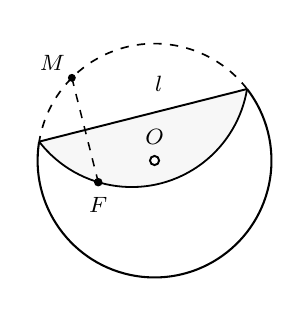
\begin{tikzpicture}[scale=1.1]
      % 圆心 O=(0,0), R=1.35, F=(-0.65, -0.25), M 在 135 度
      % 折痕 l 为 MF 的垂直平分线，交外圆于 A(170.695度), B(37.695度)
      \def\R{1.35}
      \coordinate (O) at (0,0);
      \coordinate (F) at (-0.65,-0.25);
      \coordinate (M) at ({\R*cos(135)},{\R*sin(135)});
      \coordinate (A) at ({\R*cos(170.695)},{\R*sin(170.695)});
      \coordinate (B) at ({\R*cos(37.695)},{\R*sin(37.695)});

      % 外圆周：保留部分为实线，A、B 之间被翻折走的左上圆弧为虚线
      \draw[line width=0.75pt] (A) arc[start angle=170.695, end angle=397.695, radius=\R];
      \draw[dashed, line width=0.6pt] (B) arc[start angle=37.695, end angle=170.695, radius=\R];
      % 折起弓形区域：浅灰背面填充（与图 1.1 一致）及折痕、翻折弧
      \fill[gray!6] (A) arc[start angle=-142.305, end angle=-9.305, radius=\R] -- (A) -- cycle;
      \draw[line width=0.7pt] (A) -- (B);
      \draw[line width=0.65pt] (A) arc[start angle=-142.305, end angle=-9.305, radius=\R];
      % 虚线 MF
      \draw[dashed, line width=0.55pt] (M) -- (F);

      % 标记点
      \draw[fill=white, line width=0.7pt] (O) circle (1.5pt) node[above=2pt] {\footnotesize $O$};
      \fill (F) circle (1.4pt) node[below=2pt] {\footnotesize $F$};
      \fill (M) circle (1.3pt) node[above left=-1pt] {\footnotesize $M$};
      \node[above] at (0.05,0.68) {\footnotesize $l$};
    \end{tikzpicture}
    \par\vspace{4pt}{\footnotesize 图\ 2.1}
  \end{minipage}
  \hfill
  \begin{minipage}[t]{0.47\textwidth}
    \centering
    \begin{tikzpicture}[scale=1.1]
      \def\R{1.35}
      \coordinate (O) at (0,0);
      \coordinate (F) at (-0.75,-0.1);
      \draw[line width=0.75pt] (O) circle (\R);
      \begin{scope}
        \clip (O) circle (\R);
        \foreach \ang in {10, 30, 50, 70, 90, 110, 130, 150, 170, 190, 210, 230, 250, 270, 290, 310, 330, 350} {
          \pgfmathsetmacro{\mx}{\R*cos(\ang)}
          \pgfmathsetmacro{\my}{\R*sin(\ang)}
          \pgfmathsetmacro{\kx}{0.5*(\mx - 0.75)}
          \pgfmathsetmacro{\ky}{0.5*(\my - 0.1)}
          \pgfmathsetmacro{\dx}{-(\my + 0.1)}
          \pgfmathsetmacro{\dy}{\mx + 0.75}
          \draw[line width=0.45pt, black!80]
            (\kx - 2.2*\dx, \ky - 2.2*\dy) -- (\kx + 2.2*\dx, \ky + 2.2*\dy);
        }
      \end{scope}
      \draw[line width=0.9pt, curveblue, rotate around={7.595:(-0.375,-0.05)}]
        (-0.375,-0.05) ellipse [x radius=0.675, y radius=0.559];
      \draw[fill=white, line width=0.7pt] (O) circle (1.4pt) node[below=1pt] {\footnotesize $O$};
      \draw[fill=white, line width=0.7pt] (F) circle (1.4pt) node[below=1pt] {\footnotesize $F$};
    \end{tikzpicture}
    \par\vspace{4pt}{\footnotesize 图\ 2.2}
  \end{minipage}
\end{center}

为什么这样画出的曲线一定是椭圆呢？读者可以仿照上一节自己证证看。我们只是把证明需要的辅助图形画成图 2.3，并且告诉你 $F$ 与 $O$ 正是椭圆的焦点。

\begin{center}
  \begin{tikzpicture}[scale=1.02]
    \def\R{1.35}
    \coordinate (O) at (0,0);
    \coordinate (F) at (-0.65,-0.25);
    \coordinate (M) at ({1.35*cos(140)},{1.35*sin(140)});
    \coordinate (A) at (-1.3430, 0.1367);
    \coordinate (B) at (0.9752, 0.9333);
    \coordinate (P) at (-0.5059, 0.4245);
    \coordinate (Q) at (0.1187, 0.6390);

    \draw[line width=0.75pt] (O) circle (\R);
    \draw[line width=0.7pt] (A) -- (B);
    \draw[line width=0.55pt] (M) -- (O);
    \draw[dashed, line width=0.55pt] (M) -- (F);
    \draw[line width=0.55pt] (P) -- (F);
    \draw[line width=0.55pt] (Q) -- (F);
    \draw[line width=0.55pt] (Q) -- (M);
    \draw[line width=0.55pt] (Q) -- (O);

    \fill (F) circle (1.2pt) node[below=1pt] {\footnotesize $F$};
    \fill (O) circle (1.2pt) node[below right=-1pt] {\footnotesize $O$};
    \fill (P) circle (1.2pt);
    \node[fill=white, inner sep=0.4pt] at ($(P)+(0.07,0.14)$) {\footnotesize $P$};
    \fill (Q) circle (1.2pt) node[above=1pt] {\footnotesize $Q$};
    \node[above left=-1pt] at (M) {\footnotesize $M$};
    \node[above] at (0.55,0.85) {\footnotesize $l$};
  \end{tikzpicture}
  \par\vspace{4pt}{\footnotesize 图\ 2.3}
\end{center}
